\documentclass{book}

\usepackage{graphicx}
\usepackage[italian]{babel}
%\usepackage{listings}
%\usepackage[export]{adjustbox}
\usepackage{hyperref}
\hypersetup{linktoc=all}

\begin{document}

\title{Sistemi}
\author{Giovanni Tosini}
\date{ }
\maketitle
\newpage
\tableofcontents
\newpage

\section{Numeri complessi}

Un numero complesso $s = \sigma + j\omega$ con $j = \sqrt{-1}$ e $\sigma , \omega \in R$ in cui 
\begin{itemize}
    \item $\sigma = Re(s)$ parte reale
    \item $\omega = Im(s)$ parte immaginaria
    \item $C = {s t.c. s = \sigma + j\omega, \sigma , \omega \in R}$ insieme dei numeri complessi
\end{itemize}
\begin{center}
    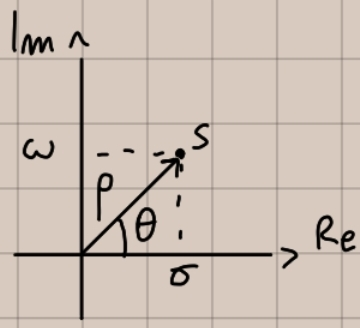
\includegraphics[width=0.5\textwidth]{num_comp.jpg}
\end{center}
Forma polare dei numeri complessi, $s = \rho (cos\theta +jsin\theta)$
\begin{itemize}
    \item $\rho = \sqrt{\sigma ^2+\omega ^2}$ il modulo di $s$ con $\rho \in R^+$
    \item $\theta =$ argomento di $s$
\end{itemize}
\begin{description}
    \item[Osservazione 1] $Re(s) = \rho cos\theta$ e $Im(s) = \rho sin\theta$
    \item[Osservazione 2] L'argomento $\theta$ è determinato a meno di multipli interi di 
            $2\pi$. Imponendo $\theta \in [0, 2\pi )$ oppure $(-\pi , \pi ]$ (deve essere un intervallo
            lungo $2\pi$ ) si ottiene l'argomento principale $\theta$ che notiamo con $arg(s)$  
\end{description}

\subsection{Formula di Eulero}

$\theta \in R, j = \sqrt{-1}$ abbiamo $e^{j\theta}=cos\theta +jsin\theta$

\paragraph{Forma esponenziale}

$s=\rho e^{j\theta}$
\begin{center}
    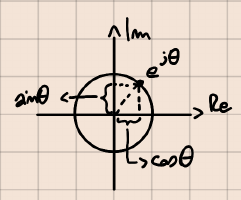
\includegraphics[width=0.5\textwidth]{num_comp2.png}
\end{center}
$|e^{j\theta}=\sqrt{cos^2\theta +sin^2\theta} = 1$

Esempio: $e^{j\frac{\pi}{2}}=j$
\begin{center}
    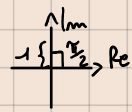
\includegraphics[width=0.5\textwidth]{num_comp3.png}
\end{center}
$s=0+1j=j$
\begin{description}
    \item[Def:] i numeri \textbf{immaginari puri} hanno la parte reale nulla
    \item[Def:] dato $s: \sigma + j\omega \in C$ $\bar{s}: \sigma - j\omega$ coniugato complesso   
\end{description}
\begin{center}
    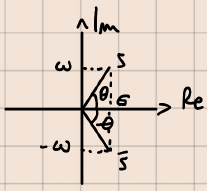
\includegraphics[width=0.5\textwidth]{num_comp4.png}
\end{center}
La forma polare di $\bar{s}$ sarà uguale a $\rho (cos\theta - jsin\theta)$
\begin{description}
    \item[Osservazione] $|s|=|\bar{s}| arg(\bar{s})=-arg(s)$ 
\end{description}

Esempio: $e^{j\pi}=-1=e^{j\pi}+1=0$
\begin{center}
    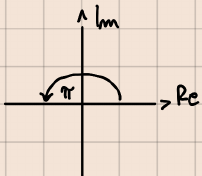
\includegraphics[width=0.5\textwidth]{num_comp5.png}
\end{center}

\subsection{Operazioni con i numero complessi}

\begin{itemize}
    \item $s_1=\sigma_1+j\omega_1,s_2=\sigma_2+j\omega_2\in C$
    \item $s_1+s_2=\sigma_1+\sigma_2+j(\omega_1+\omega_2)$
    \item $s_1-s_2=\sigma_1-\sigma_2+j(\omega_1-\omega_2)$
\end{itemize}
\begin{description}
    \item[Osservazione:] $Re(s)=\frac{s+\bar{s}}{2}$ e $Im(s)=\frac{s+\bar{s}}{2j}$ 
\end{description}
Per la formula di Eulero $e^{j\theta}=cos\theta+jsin\theta \Rightarrow cos\theta = \frac{e^{j\theta}+e^{-j\theta}}{2}$ e
$sin\theta =\frac{e^{j\theta} -e^{-j\theta}}{2j}$
\begin{center}
    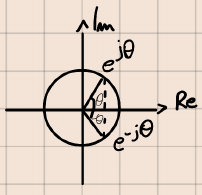
\includegraphics[width=0.5\textwidth]{num_comp6.png}
\end{center}
\begin{description}
    \item[Osservazione:]$2Re(s)=s+\bar{s}$ e $2jIm(s)=s-\bar{s}$ 
\end{description}
$s=\bar{s} \Rightarrow Im(s)=0$ e $s=-\bar{s} \Rightarrow Re(s)=0$
\begin{center}
    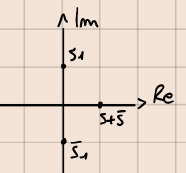
\includegraphics[width=0.5\textwidth]{num_comp7.png}
    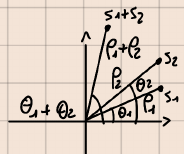
\includegraphics[width=0.5\textwidth]{num_comp8.png}
\end{center}
\begin{itemize}
    \item $s_1 = \rho_1(cos\theta_1+jsin\theta_1)$
    \item $s_2 = \rho_1(cos\theta_2+jsin\theta_2)$
    \item $s_1s_2=\rho_1\rho_2(cos(\theta_1+\theta_2)+jsin(\theta_1+\theta_2))$
    \item $s_1s_2=\rho_1\rho_2(cos\theta_1cos\theta_2+jcos\theta_1sin\theta_2+jsin\theta_1cos\theta_2-sin\theta_1sin\theta_2)$
    \item $s_1s_2=\rho_1\rho_2(cos\theta_1cos\theta_2-sin\theta_1sin\theta_2+j(cos\theta_1sin\theta_2+sin\theta_1cos\theta_2))$
\end{itemize}
\begin{description}
    \item[N.B.:] $cos\theta_1cos\theta_2-sin\theta_1sin\theta_2=cos(\theta_1+\theta_2)$ e 
    $cos\theta_1sin\theta_2+sin\theta_1cos\theta_2=sin(\theta_1+\theta_2)$
    \item [Def:]Dato $s\in C$ il numero $s^{-1}$ t.c. $ss^{-1}=1$, $s^{-1}=\frac{\bar{s}}{|s|^2}$ reciproco
    (inverso) di $s$.
    \item $ss^{-1}=s\frac{\bar{s}}{|s|^2}=\frac{s\bar{s}}{|s|^2}$
    \item $s\bar{s}=\rho^2(cos(\theta-\theta)+jsin(\theta-\theta))=\rho^2=|s|^2$
    \item [Osservazione:]l'argomento di un numero complesso si può chiamare anche \textbf{fase}.
    \item $\frac{s_1}{s_2}=s_1s_2^{-1}=s_1\frac{\bar{s_2}}{|s_2|^2}=\frac{\rho_1}{\rho_2}(cos(\theta_1-\theta_2)
    jsin(\theta_1-\theta_2))$
    \item [Osservazione:] $s\bar{s}=\rho^2(cos(\theta-\theta)+jsin(\theta-\theta))=\rho^2\Rightarrow|s|^2=s\bar{s}$ 
\end{description}
\begin{center}
    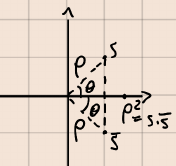
\includegraphics[width=0.5\textwidth]{num_comp9.png}
\end{center}
\begin{description}
    \item[Def: ]$u\in C$ si dice complesso unitario se $|u|=1$. In forma polare $u=cos\theta+jsin\theta$. In forma esponenziale
     $u=e^{j\theta}$ e $|e^{j\theta}|=1$  
\end{description}
Sia $u=cos\alpha+jsin\alpha$ con $s=\rho(cos\theta+jsin\theta)$ avremo che $su=\rho(cos(\theta+\alpha)+jsin(\theta+\alpha))$
(rotazione intorno all'origine)
\begin{center}
    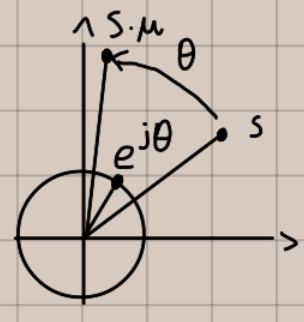
\includegraphics[width=0.5\textwidth]{num_comp10.jpg}
\end{center}
$s^n=\rho^n(cos(n\theta)+jsin(n\theta))$

Esempio: $(e^{j\theta})^n=e^{jn\theta}$

\paragraph{Radici complesse}

Ogni $s\in C$ ammette $n$ distinte radici $n$-esime $\omega_1,...,\omega_{n-1} \in C$.
Dobbiamo trovare $\omega \in C$ t.c. $\omega^n=s$.
\newline $\forall k \in [0, n-1], \omega_k\sqrt[n]{\rho}(cos(\frac{\theta}{n}+\frac{2\pi}{n}k)
+jsin(\frac{\theta}{n}+\frac{2\pi}{n}k))$
\newline Prova: $\omega_k^n=(\sqrt[n]{\rho}^n)(cos(n(\frac{\theta}{n}+\frac{2\pi}{n}k))+jsin(n(\frac{\theta}{n}+\frac{2\pi}{n}k)))$
\newline $\rho(cos(\theta+2\pi k)+jsin(\theta+2\pi k))=s$
\newline Notare che $cos(\theta+2\pi k)$ è equivalente a $cos\theta$ e $sin(\theta+2\pi k)$ equivale a $sin\theta$ questo
$\forall k=0,...,n-1 $

L'equazione: $s^4=1+2j$ ha 4 radici distinte nel campo $C$.
Esempio: le radici complesse dell'unità

$s^n=1 \omega_k=cos(\frac{2\pi}{n}k) + jsin(\frac{2\pi}{n}k) k=0,...,n-1$

\paragraph{Funzioni di variabile complessa}

Gli insieme su cui definiamo una funzione di variabile complessa
 f si scrivono $D(f)$, $D(f)\subseteq C$
 \begin{description}
     \item[Def: ]un punto $s_0\in D(f)\subseteq C$ è interno a $D(f)$
     se esiste un disco $B_\rho(s_0)$ di raggio $\rho$ con $\rho\in R^+$ centrato
     in $s_0$, t.c. $B_\rho(s_0)\subseteq D(f)$ dove $B_\rho(s_0)={s\in C t.c. |s-s_0| < \rho}$
 \end{description}
 \begin{center}
     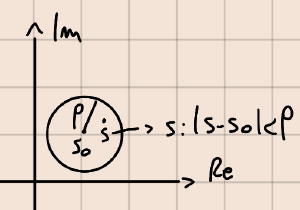
\includegraphics[width=0.5\textwidth]{num_comp11.png}
 \end{center}
 \begin{description}
     \item[Def: ]Un insieme $D(f)\subseteq C$ si dice aperto se tutti i suoi punti
     sono interni 
     \item [Def: ]Una funzione $f:D(f)\rightarrow C$ con $D(f)\subseteq C$ aperto
     è una funzione complessa
 \end{description}
 Esempi di funzioni complesse con annesso dominio:
 \begin{itemize}
     \item $f(s) = s, D(f) = C$
     \item $f(s)=s^2,D(f)=C$
     \item $f(s)=Re(s)+jIm(s)^2, D(f)=C$
     \item $f(s)=\sum_{k=0}^n a_ks^k, D(f)=C$
     \item funzione polinomiale, $f(s)=\frac{P(s)}{Q(s)}$ dove $P(s)=\sum_{k=0}^n a_ks^k$ e funzione razionale $Q(s)=\sum_{k=0}^n b_ks^k$,
     $D=C-{\lambda_1,...,\lambda_m}$ dove $\lambda_\alpha$ è radice di $Q(s)=0$ per $k=1,...,m$
 \end{itemize}
 \subsection{Teorema fondamentale dell'algebra}
 Ogni polinomio $P(s)$ a coefficienti complessi di grado $n>0$ ha $n$ radici complesse e si può comporre come
 \begin{center}
         $P(s) = a_n(s-\lambda_1)^\mu_1(s-\lambda_2)^\mu_2...(s-\lambda_r)^\mu_r$ dove 
        $\lambda_1,...\lambda_r$ sono radici  e $\mu_1,...,\mu_r$ sono le \textbf{molteplicità} relative di ciascuna
        radice per cui $\mu_1 + ... + \mu_r = n$
 \end{center}
 \begin{description}
     \item[Osservazione] Un numero $\lambda$ è una radice di molteplicità $\mu$ per un polinomio $P(s)$
    se e solo se $P(\lambda)=P'(\lambda)=P''(\lambda)=...=P^{\mu - 1}(\lambda) = 0$ e $P^\mu (\lambda)\neq 0$
    \end{description}


    
\end{document}